%!TEX root = ../thesis.tex
%*******************************************************************************
%********************************* Seventh Chapter *****************************
%*******************************************************************************
\cleardoublepage
\chapter{Application to wind turbine fatigue reliability and robustness}
\label{chpt:7}
%*******************************************************************************
\hfill
\localtableofcontents
\newpage



\elias{https://www.sciencedirect.com/science/article/pii/S136403212200171X}

\elias{https://doi.org/10.1016/j.ijfatigue.2020.105487}

\elias{https://doi.org/10.1016/j.ress.2019.106550}

%============================================================%
%============================================================%
\section{Introduction}
%============================================================%
%============================================================%
One of the main goals of this work is to evaluate the reliability of an OWT's monopile foundation with respect to fatigue solicitations. 
Let us recall the usual approach to assess fatigue damage over the structure's lifetime (see \citealp[Appendix H]{iec_2019}). 
First, the lifetime duration $T$ is discretized into $N_T \in \N$ 10-minutes intervals $\{t^{(i)}\}_{i=1}^{N_T}$. 
The 10-minutes duration results from the typical wind energy distribution (see \fig{fig:wind_psd}), presenting a ``short-term'' behavior (for turbulent wind with a return period below 10 minutes) and ``long-term'' behavior (otherwise).
Then the environmental conditions can be considered as a stochastic process $\{\bX(t, \omega), \, t \in T, \, \omega \in \Omega\}$ \elias{illustrated in \fig{fig:wind_long_short_term}}. 
For a realization $\bX(t^{(i)}, \omega^{(r)})$ and a given set of parameters $z$ related to the system (defined in Table~\ref{tab:sys_variables}), one can perform a 10-minutes Turbsim-DIEGO simulation and post-process it (see Section~\ref{sec:235}) to obtain a corresponding cumulative damage:
\begin{equation}
    d_{\mathrm{c}}^{10\mathrm{min.}}(\bX(t^{(i)}, \omega^{(r)})|Z=z). 
\end{equation}
To cumulate the damage over the lifetime, let us write the sum of 10-minutes damages, each averaged over $n_{\mathrm{rep}} \in \N$ pseudo-random seed repetitions: 
\begin{subequations}
    \begin{align}
        D(z) &= \frac{1}{n_{\mathrm{rep}}} \, \sum_{i=1}^{N_T} \sum_{r=1}^{n_{\mathrm{rep}}} d_{\mathrm{c}}^{10\mathrm{min.}}(\bX(t^{(i)}, \omega^{(r)})|Z=z)\\
             &= N_T \frac{1}{N_T \, n_{\mathrm{rep}}} \, \sum_{i=1}^{N_T} \sum_{r=1}^{n_{\mathrm{rep}}} d_{\mathrm{c}}^{10\mathrm{min.}}(\bX(t^{(i)}, \omega^{(r)})|Z=z)\\
             &\approx N_T \, \E_{\bX}\left[d_{\mathrm{c}}^{10\mathrm{min.}}(\bX|Z=z)\right],
             \label{eq:expected_damage}
    \end{align}
\end{subequations}
where $\bX \sim f_\bX$ is the random vector of the long-term environmental conditions, defined in Table~\ref{tab:envi_variables}. 

In Chapter~\ref{chpt:4}, kernel herding was proposed as a method for given-data subsampling to propagate the uncertain environmental conditions on Teesside's OWT model. 
This method showed equivalent performances to quasi-Monte Carlo for estimating the lifetime damage in \eq{eq:expected_damage}, while being more flexible. 
In the linear cumulative damage model considered by the community (Miner's rule), a damage value higher than one leads to fatigue failure by convention. 
The present chapter assesses the probability of such rare event, considering both the environmental uncertainties (aggregated according to \eq{eq:expected_damage}) and the uncertainties related to the system itself (described by the random variable $\bZ \in \iD_\bZ$ with PDF $f_\bZ$). 
Assuming that the critical damage $D_{\mathrm{cr}}$ is a random variable centered around one (equivalent to a ``resistance'' variable in reliability analysis), this failure probability is written:
\begin{equation}
    \pf = \int_{\iD_\bZ} \1_{\{D(\bz) \geq D_{\mathrm{cr}}\}} \, f_\bZ(\bz) \, \dd z \,.
    \label{eq:owt_pf}
\end{equation}

Less information is available to define the probabilistic model of the system uncertainties than the environmental uncertainties. 
%For example, the soil geotechnical properties are by nature hard to measure without  
Therefore, the robustness of the failure probability to the probabilistic model $\bZ$ should be studied. 
To do so, a perturbation-based approach called the \textit{perturbed-law based sensitivity indices} (PLI) is used in this chapter \citep{lemaitre_2015_PLI}.   

The present chapter is structured as follows: 
Section~\ref{sec:owt_surrogate} presents the construction of a surrogate model of $D(\cdot)$,
then Section~\ref{sec:owt_ra} analyses the reliability of the monopile foundation of Teesside's turbine for a nominal distribution of $\bZ$, 
and finally Section~\ref{sec:owt_robustness} proposes a robustness analysis of $\pf$ by perturbing the law of $\bZ$ and $D_{\mathrm{cr}}$.

%============================================================%
%============================================================%
\section{Surrogate modeling for reliability analysis}\label{sec:owt_surrogate}
%============================================================%
%============================================================%
The prohibitive computational cost of the function $D(\cdot)$ requires fitting a surrogate model.  
This section presents the specific high-performance computer (HPC) wrapper developed for this application and its use to build a learning set for a Gaussian process regression. 

%============================================================%
\subsection{High-performance computer evaluation}
%============================================================%
The wrapper of the numerical chain including Turbsim and Diego (illustrated in \fig{fig:owt_chained_model}) for reliability analysis has a nested double loop structure.  
The outer loop pilots the realizations of $\bZ$ while the inner loop concerns the environmental conditions and their repetitions with $n_{\mathrm{rep}}$ different pseudo-random seeds. 
At this stage, the goal is to approximate $\what{D}(k_{\mathrm{soil}}, \theta_{\mathrm{yaw}}):\R^2 \rightarrow \R$: 
\begin{equation}
    \what{D}(k_{\mathrm{soil}}, \theta_{\mathrm{yaw}}) = N_T \sum_{i=1}^{n_\bX} \sum_{r=1}^{n_{\mathrm{rep}}} d_{\mathrm{c}}^{10\mathrm{min.}}(\bx^{(i)}, \omega^{(r)} | K_{\mathrm{soil}}, \Theta_{\mathrm{yaw}}),
    \label{eq:hpc_cumulated_damage}
\end{equation}
where $\{\bx^{(i)}\}_{i=1}^{n_\bX}$ are defined by kernel herding, and $(K_{\mathrm{soil}}, \Theta_{\mathrm{yaw}})\TT$ are the system variables which are direct inputs of DIEGO (i.e., not part of the post-processing). 
According to the convergence results obtained in Chapter~\ref{chpt:4}, the kernel herding size is fixed at $n_\bX=200$ and the repetitions at $n_{\mathrm{rep}}=11$, which implies a total of $2200$ Turbsim-DIEGO simulations per evaluation of the function $\what{D}(\cdot)$. 
In this setup, the CRONOS HPC from EDF allows us to simultaneously perform those 2200 simulation in parallel. 
The random variable associated with the SN-curve uncertainty is introduced later as a product factor of \eq{eq:hpc_cumulated_damage}. 
Note that the cumulative damage studied is actually the maximum value of $\what{D}(\cdot)$ over the discretized azimuth angles (illustrated in \fig{fig:wind_wave_roses}), at the mudline level. 


%============================================================%
\subsection{Design of experiments}
%============================================================%

To build a learning set, a space-filling design of experiments is created on the joint domain of $(K_{\mathrm{soil}}, \Theta_{\mathrm{yaw}})$. 
This design was first composed of 30 points generated by a Halton sequence (illustrated in \fig{fig:initial_doe}.a) which was the most space-filling sequential method in two dimensions. 
Its evaluation and analysis showed that the highest damage values are the result of high yaw misalignment errors and low soil stiffness. 
Therefore, the design was completed in a second phase by 20 points targeting these areas by applying a kernel herding in a subdomain defined a priori (see the candidate set represented by the gray points in \fig{fig:initial_doe}.b). 
Finally, the learning set is the union of the two complementary designs, later referred as the ``composite design'', in reference to the heterogeneous composition of composite materials. 
This composite design, denoted by $\bZ_{n_\bZ}$, has a size of $n_\bZ=50$, which represents over $10^5$ Turbsim-DIEGO simulations (each requiring around 45 minutes of CPU time).
\fig{fig:evaluated_doe} shows the lifetime cumulated damage evaluated on the composite design (with normalized values corresponding to the color scale). 

%\elias{Comment on the fact that it's not symmetric}. 
%\elias{the damage values are obtained for a nominal SN curve defined in xxxx for Teesside's model defined in Chapter 4}


\begin{figure}
    \centering
    \begin{subfigure}{0.48\linewidth}
        \vskip -30pt
        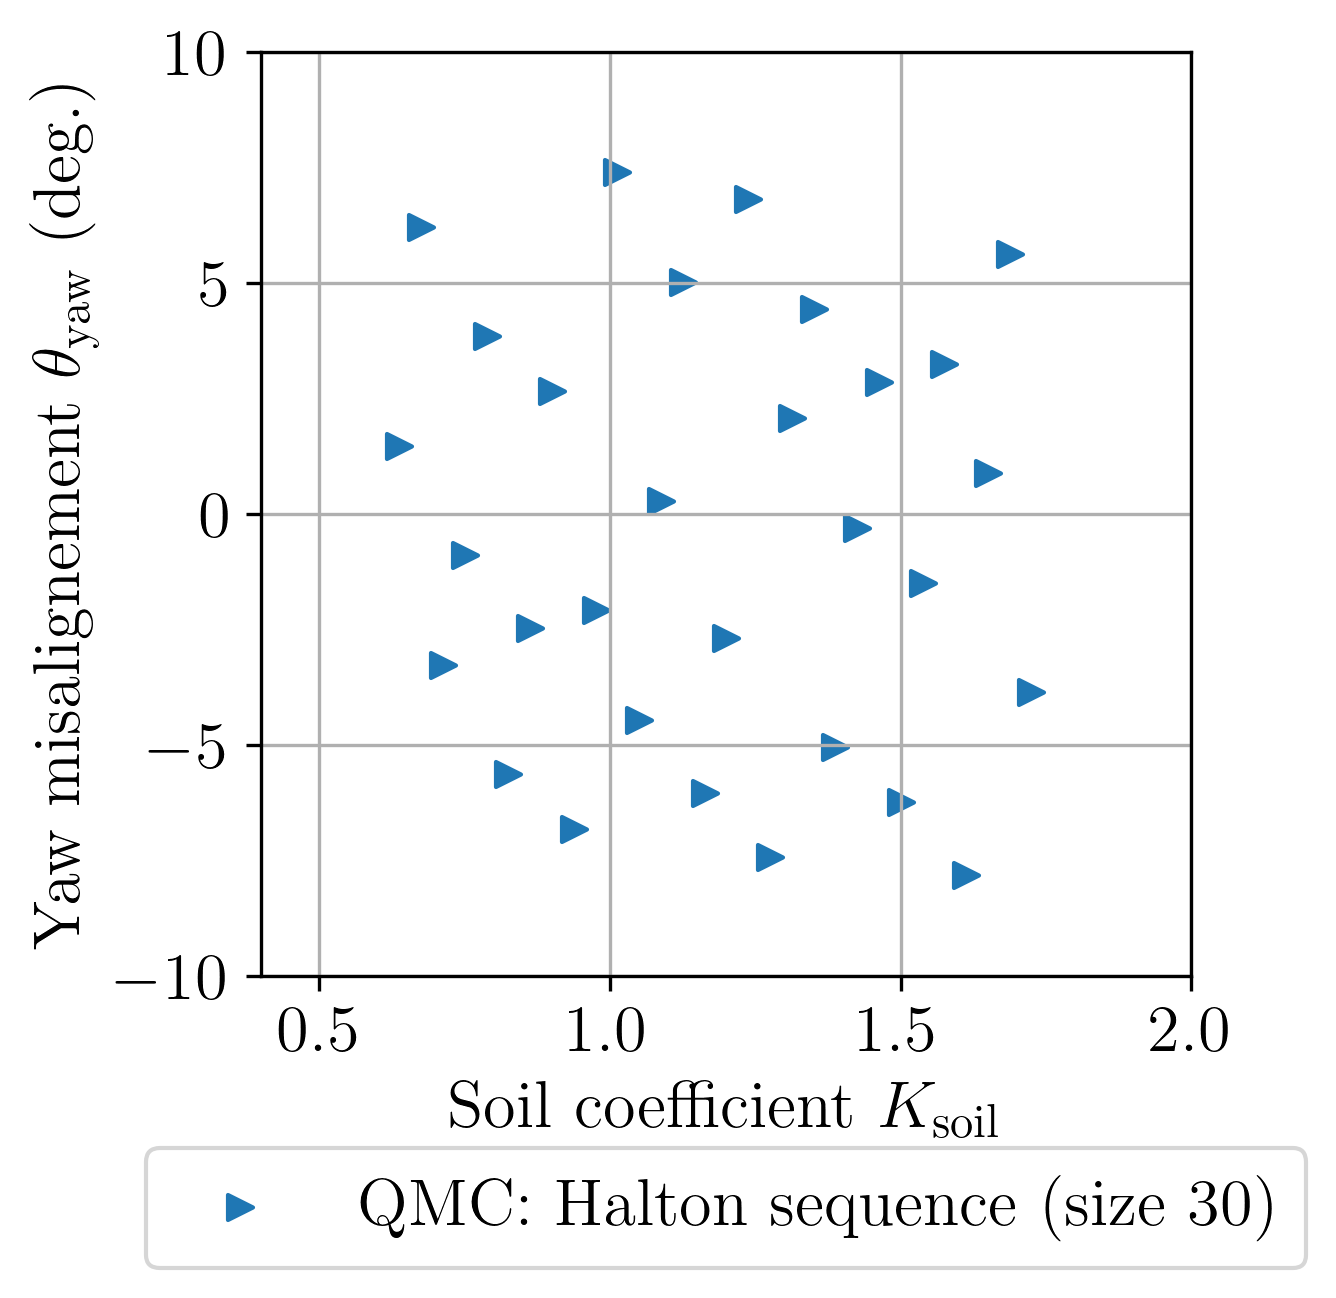
\includegraphics[width=\linewidth]{./part3/figures/OWT/initial_halton.png}
        \caption{Halton sequence.}
    \end{subfigure}
    \begin{subfigure}{0.48\linewidth}
        %\vskip 0pt
        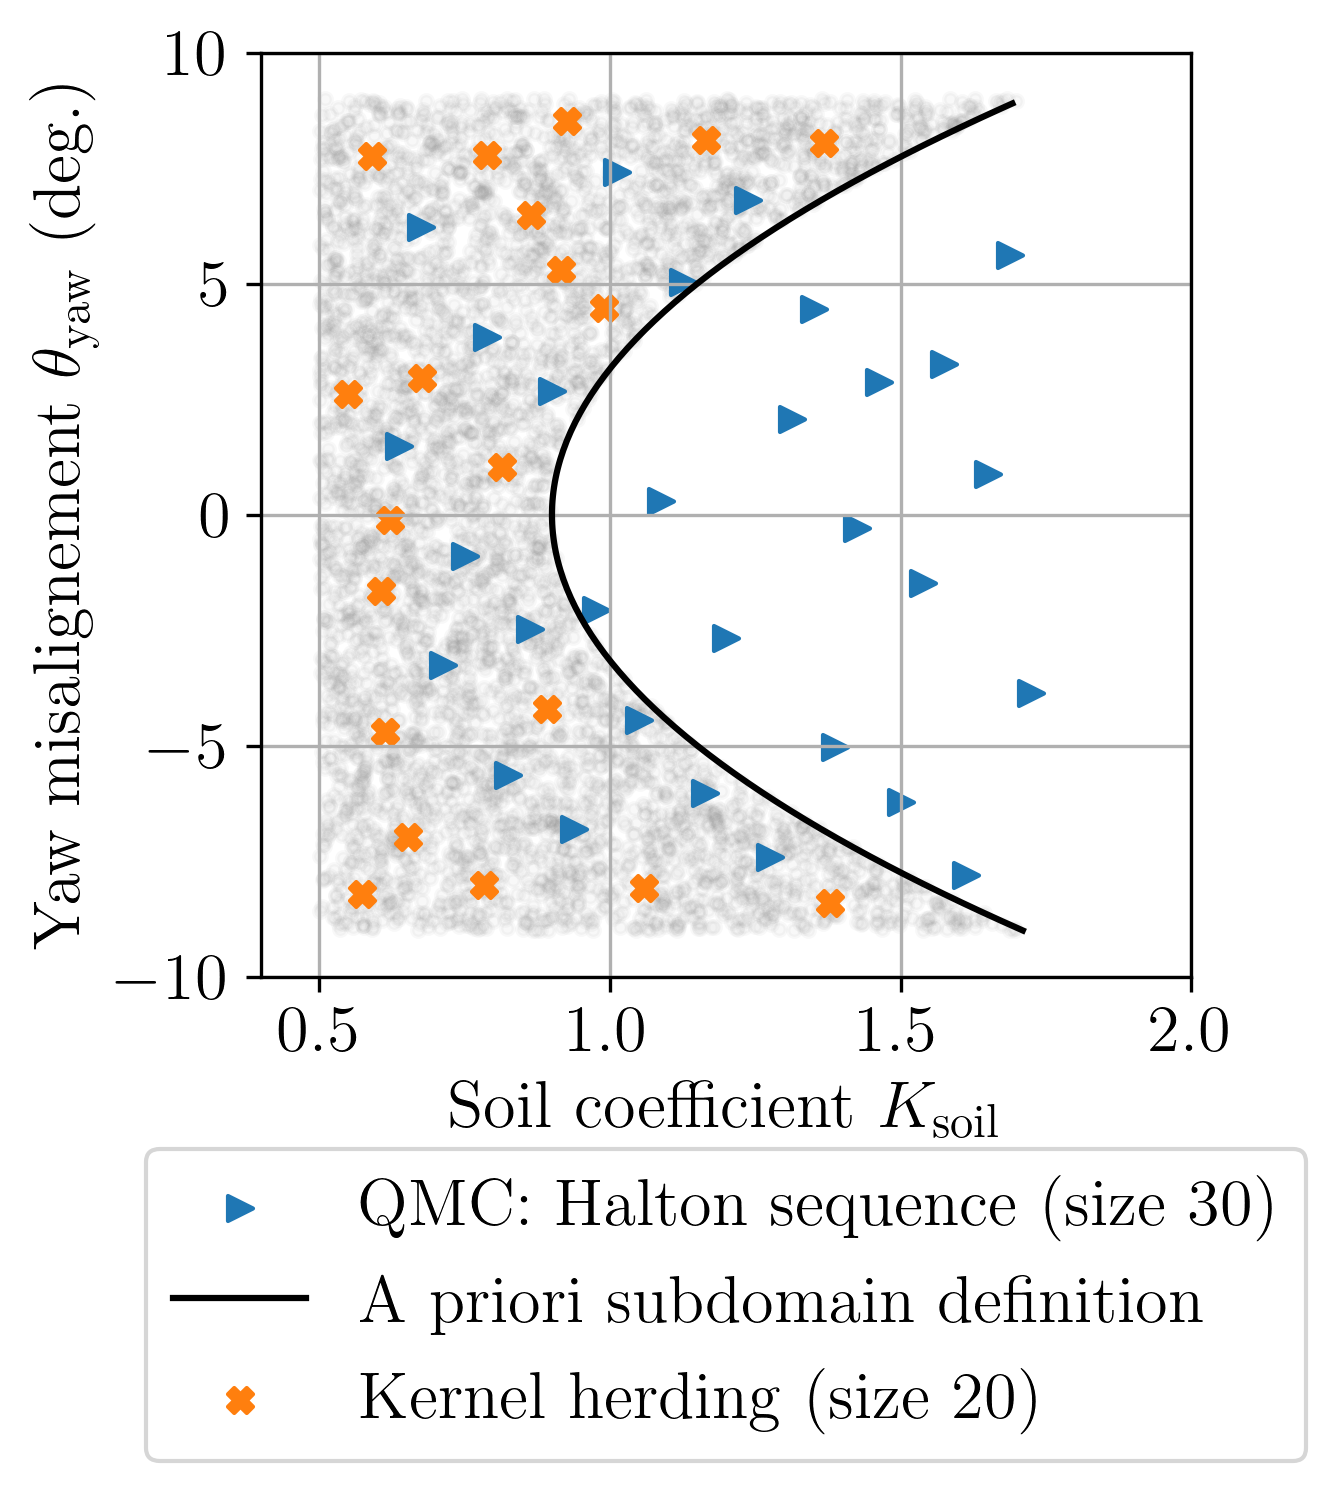
\includegraphics[width=\linewidth]{./part3/figures/OWT/initial_composite.png}
        \caption{Composite design.}
    \end{subfigure}
    \caption{Learning set of the mean damage surrogate model. A Halton sequence is first built (in blue) and competed by kernel herding points (in orange) in a subdomain defined a priori (in gray).}
    \label{fig:initial_doe}
\end{figure}

\begin{figure}[h!]
    \centering
    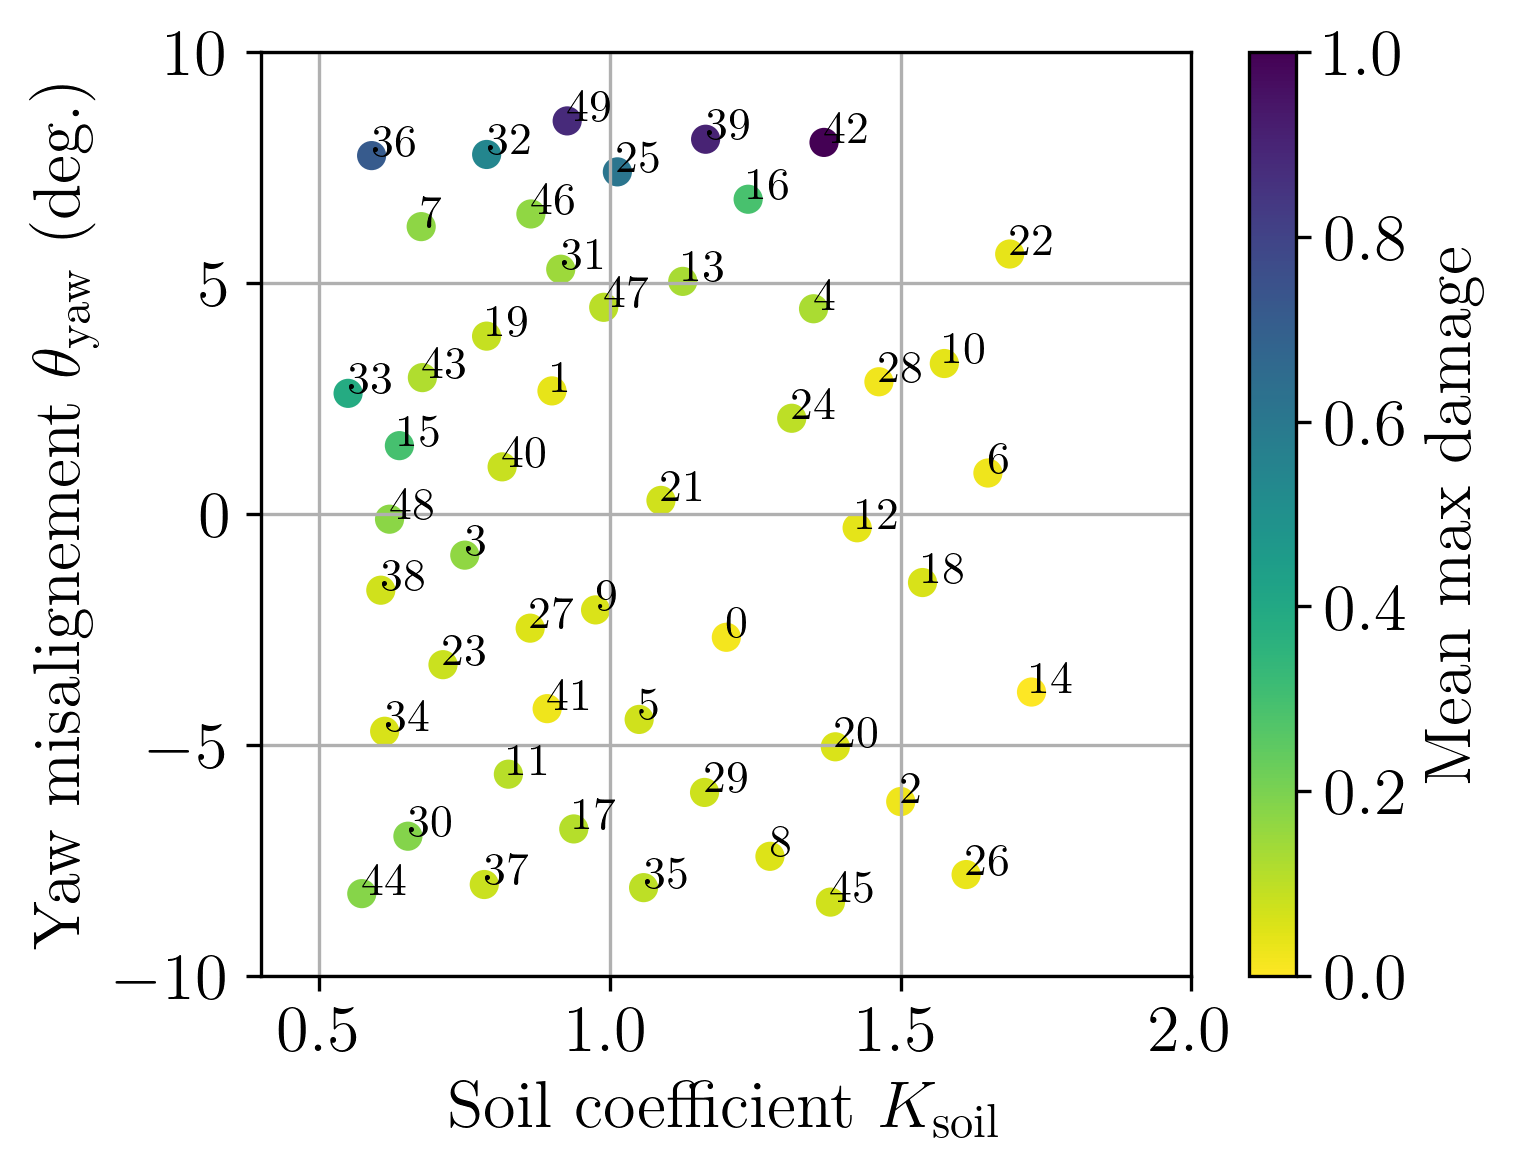
\includegraphics[width=0.6\linewidth]{./part3/figures/OWT/normalized_results_mean.png}
    \caption{Normalized mean damage evaluated on the composite design illustrated in \fig{fig:initial_doe}.b.}
    \label{fig:evaluated_doe}
\end{figure}


%============================================================%
\subsection{Gaussian process regression}
%============================================================%

A Gaussian process regression with Matérn $5/2$ and constant trend is fitted on the composited design $\bZ_{n_\bZ}$ according to the kriging equation introduced in Section~\ref{sec:surrogate}. 
The resulting surrogate model $\widetilde{D}:\R^2 \rightarrow \R$, is represented by the blue three-dimensional surface in \fig{fig:3d_owt_surrogate}, and its learning set  $\bZ_{n_\bZ}$ by the black crosses.  
A complementary visualization of this surrogate is proposed for cross-sections with fixed values $\theta_{\mathrm{yaw}}=0$ on \fig{fig:owt_surrogate}.a, and $k_{\mathrm{soil}}=1$ on \fig{fig:owt_surrogate}.b. 
On these two figures, learning points are plotted in a gray scale and the surrogate model in a blue scale. 
The darkest the shade, the closest to the cross-section the points are. 

To validate this surrogate model, a leave-one-out (LOO) procedure is realized. 
\fig{fig:loo_validation}.b represents the LOO squared-residuals at each points of the design (with values corresponding to the color scale). 
High residual values are mostly due to the strong nonlinearity of the code in some areas (as revealed by the cross-section in \fig{fig:owt_surrogate}.b).
\fig{fig:loo_validation}.a shows the quantile-quantile plot comparing the LOO predictions with the lifetime damage evaluations on the learning set. 
The general coefficient of predictivity of $\what{Q}^2_{LOO}=0.72$ is considered acceptable in this small data context, especially as the LOO procedure was shown to underestimate the true performance metric in Chapter~\ref{chpt:5}. 
However, more points could be added to complete the learning set in regions with high nonlinearities to enhance the surrogate presented.  

\begin{remark}
    ~
    \begin{itemize}
        \item Active learning methods for reliability (see Section~\ref{sec:active_surrogates}) could be a great option for such costly function. 
        However, the stochasticity of the function would disturb the learning criterion. Since the nonlinearities seem restricted to a small area, the present approach should be more robust. 
        \item Another approach could be to fit a stochastic surrogate \citep{binois_2019_replication,baker_2020_stochastic_surrogates_review,zhu_2023_thesis} on a learning set before averaging on the pseudo-random seed repetitions.  
    \end{itemize} 
\end{remark}

\begin{figure}[h!]
    \centering
    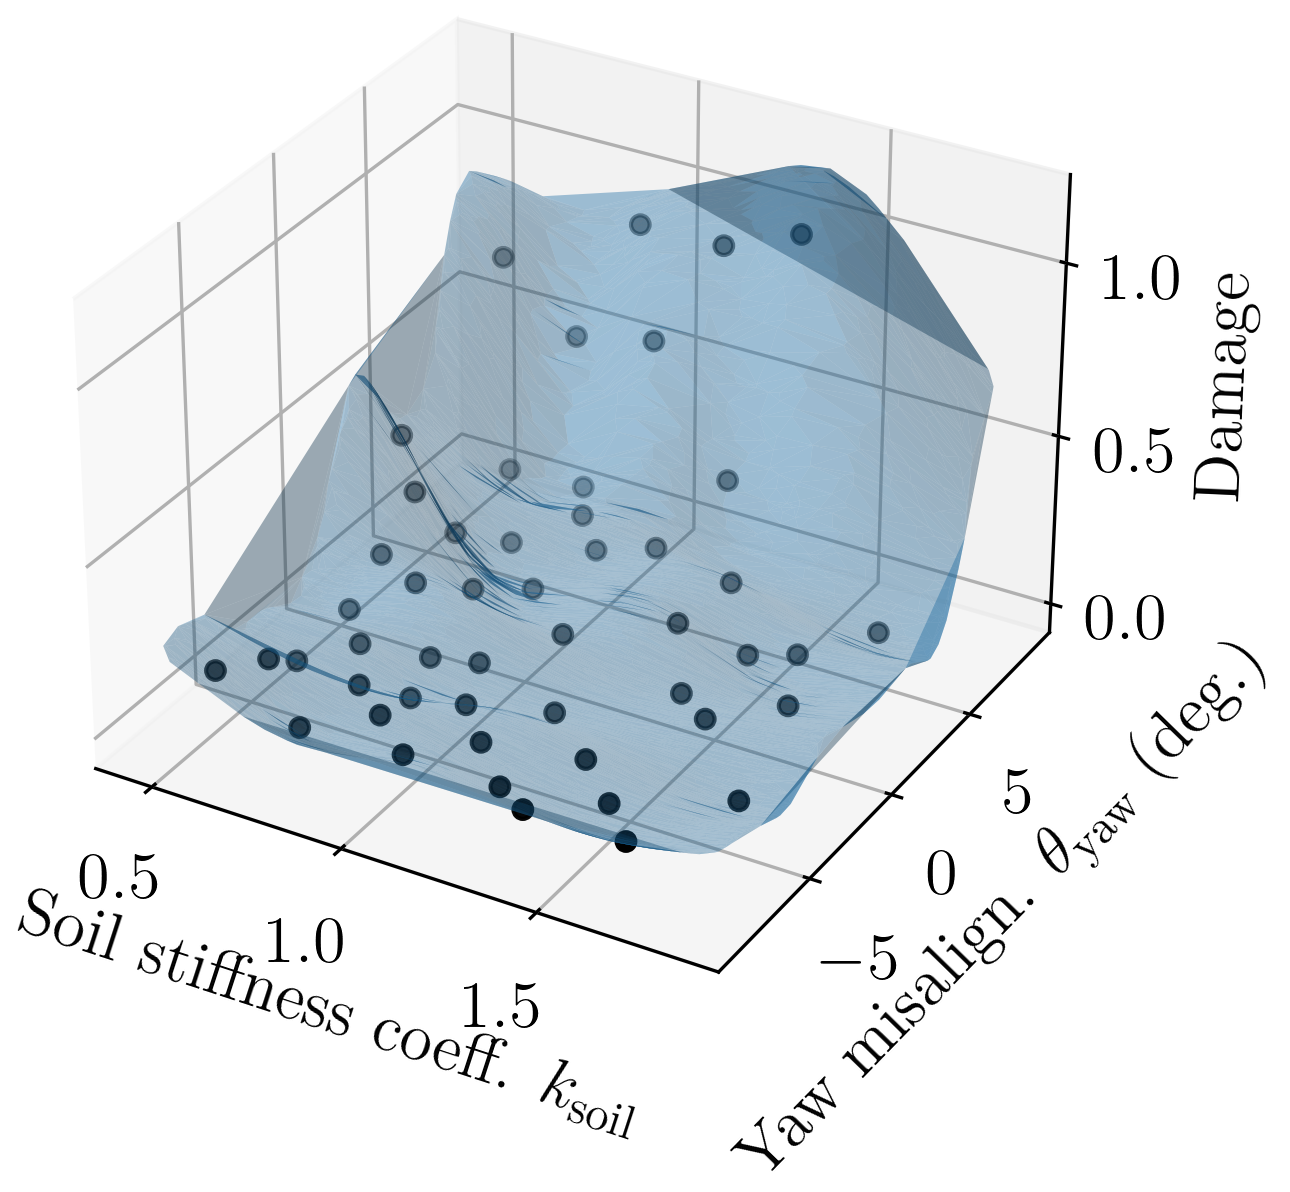
\includegraphics[width=0.45\linewidth]{./part3/figures/OWT/3D_surrogate.png}
    \caption{Three-dimensional plot of the surrogate model $\widetilde{D}$ (in blue) and learning set (in black).}
    \label{fig:3d_owt_surrogate}
\end{figure}

\begin{figure}[h!]
    \centering
    \begin{subfigure}[b]{0.38\linewidth}
        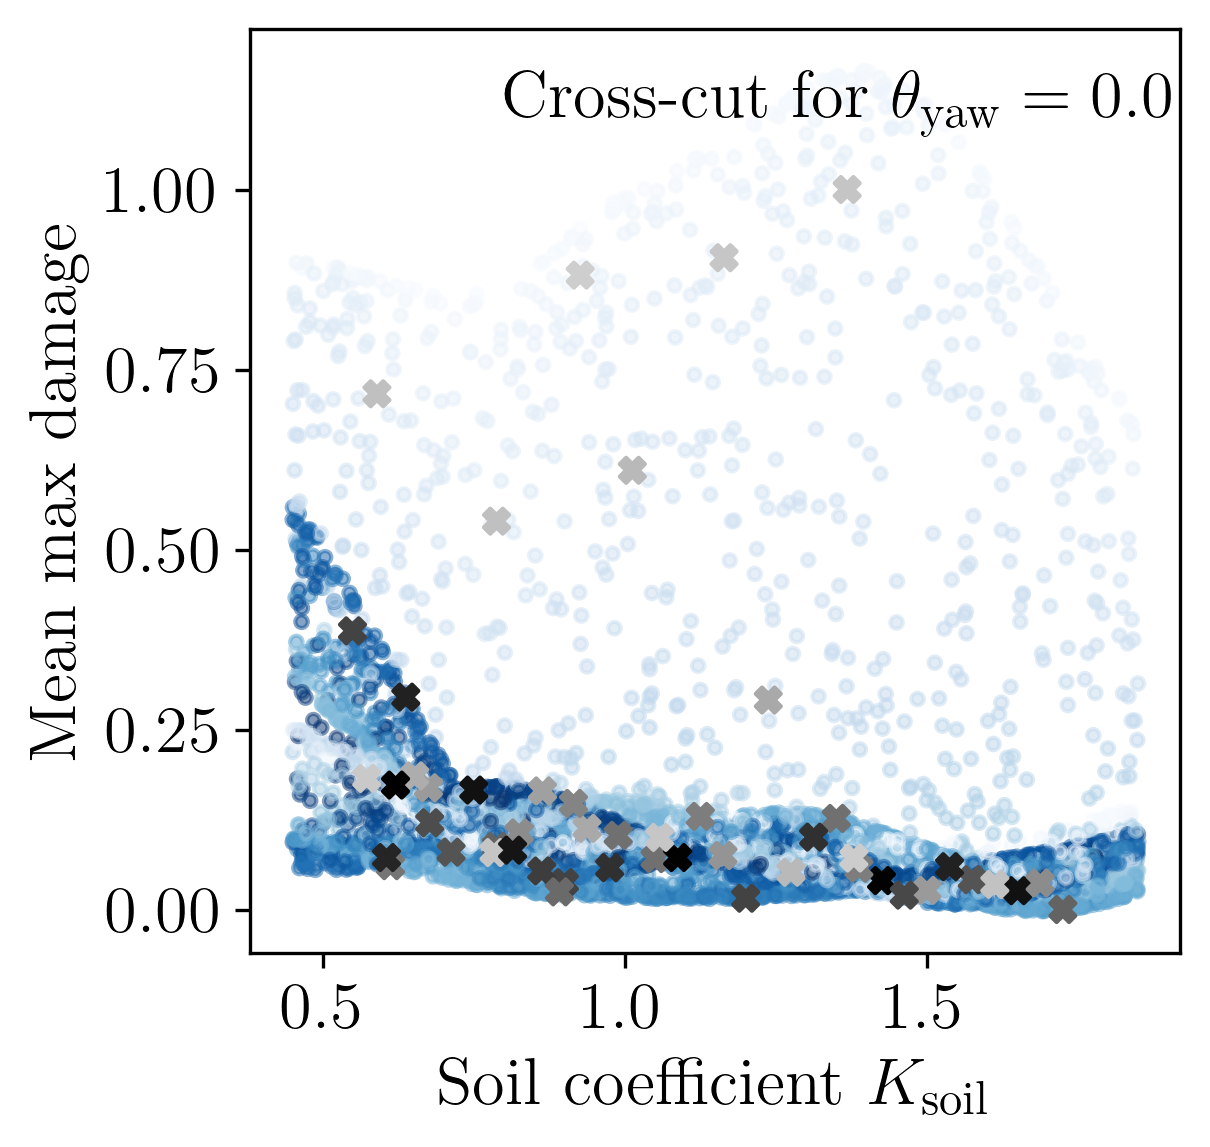
\includegraphics[width=\linewidth]{./part3/figures/OWT/dam_vs_soil_surrogate.png}
        \caption{$\theta_{\mathrm{yaw}}=0$.}
    \end{subfigure}
    \begin{subfigure}[b]{0.38\linewidth}
        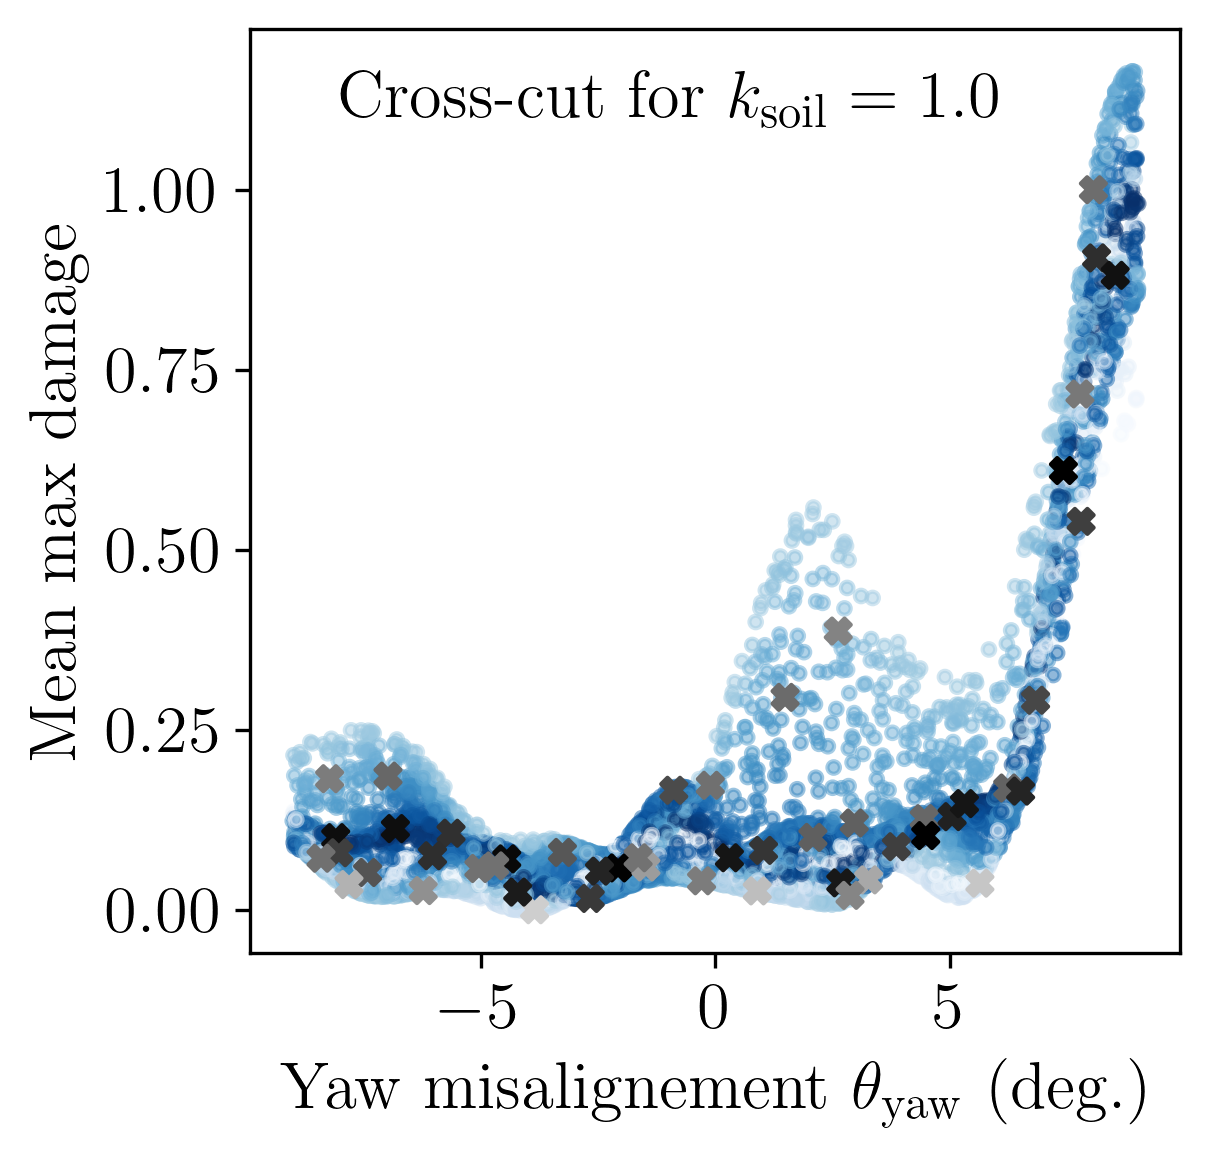
\includegraphics[width=\linewidth]{./part3/figures/OWT/dam_vs_yaw_surrogate.png}
        \caption{$k_{\mathrm{soil}}=1$.}
    \end{subfigure}
    \caption{Cross-section of the surrogate model $\widetilde{D}$ (in shades of blue) for given values of $k_{\mathrm{soil}}$ and $\theta_{\mathrm{yaw}}$. The darkest the shade, the closest to the cross-section.}
    \label{fig:owt_surrogate}
\end{figure}

\begin{figure}[h!]
    \centering
    \begin{subfigure}[t]{0.36\linewidth}
        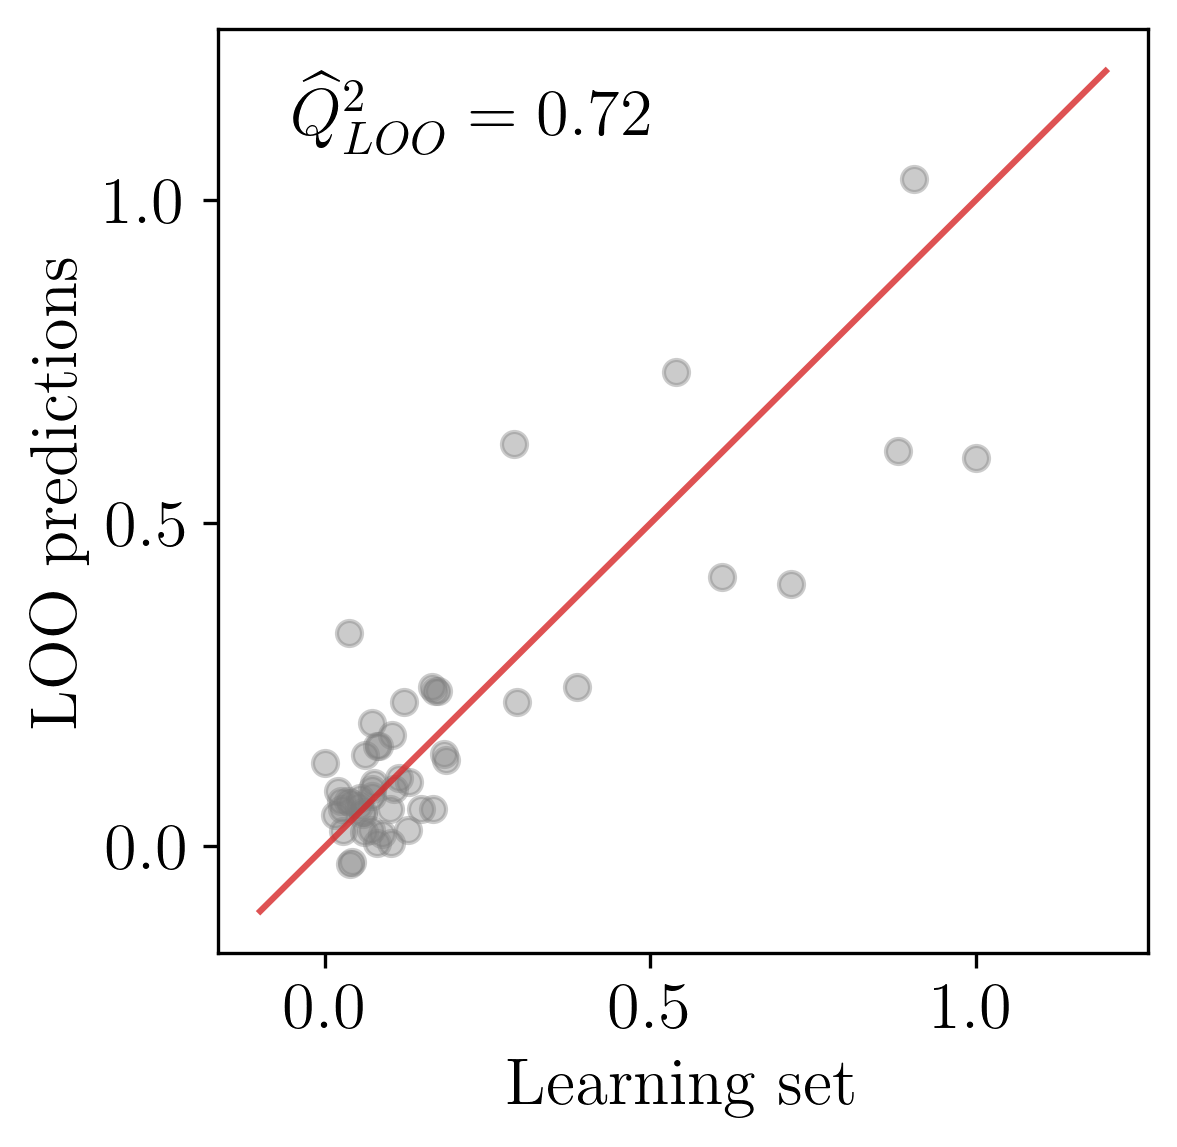
\includegraphics[width=\linewidth]{./part3/figures/OWT/loo_qqplot.png}
        \caption{Quantile-quantile plot.}
    \end{subfigure}
    \begin{subfigure}[t]{0.48\linewidth}
        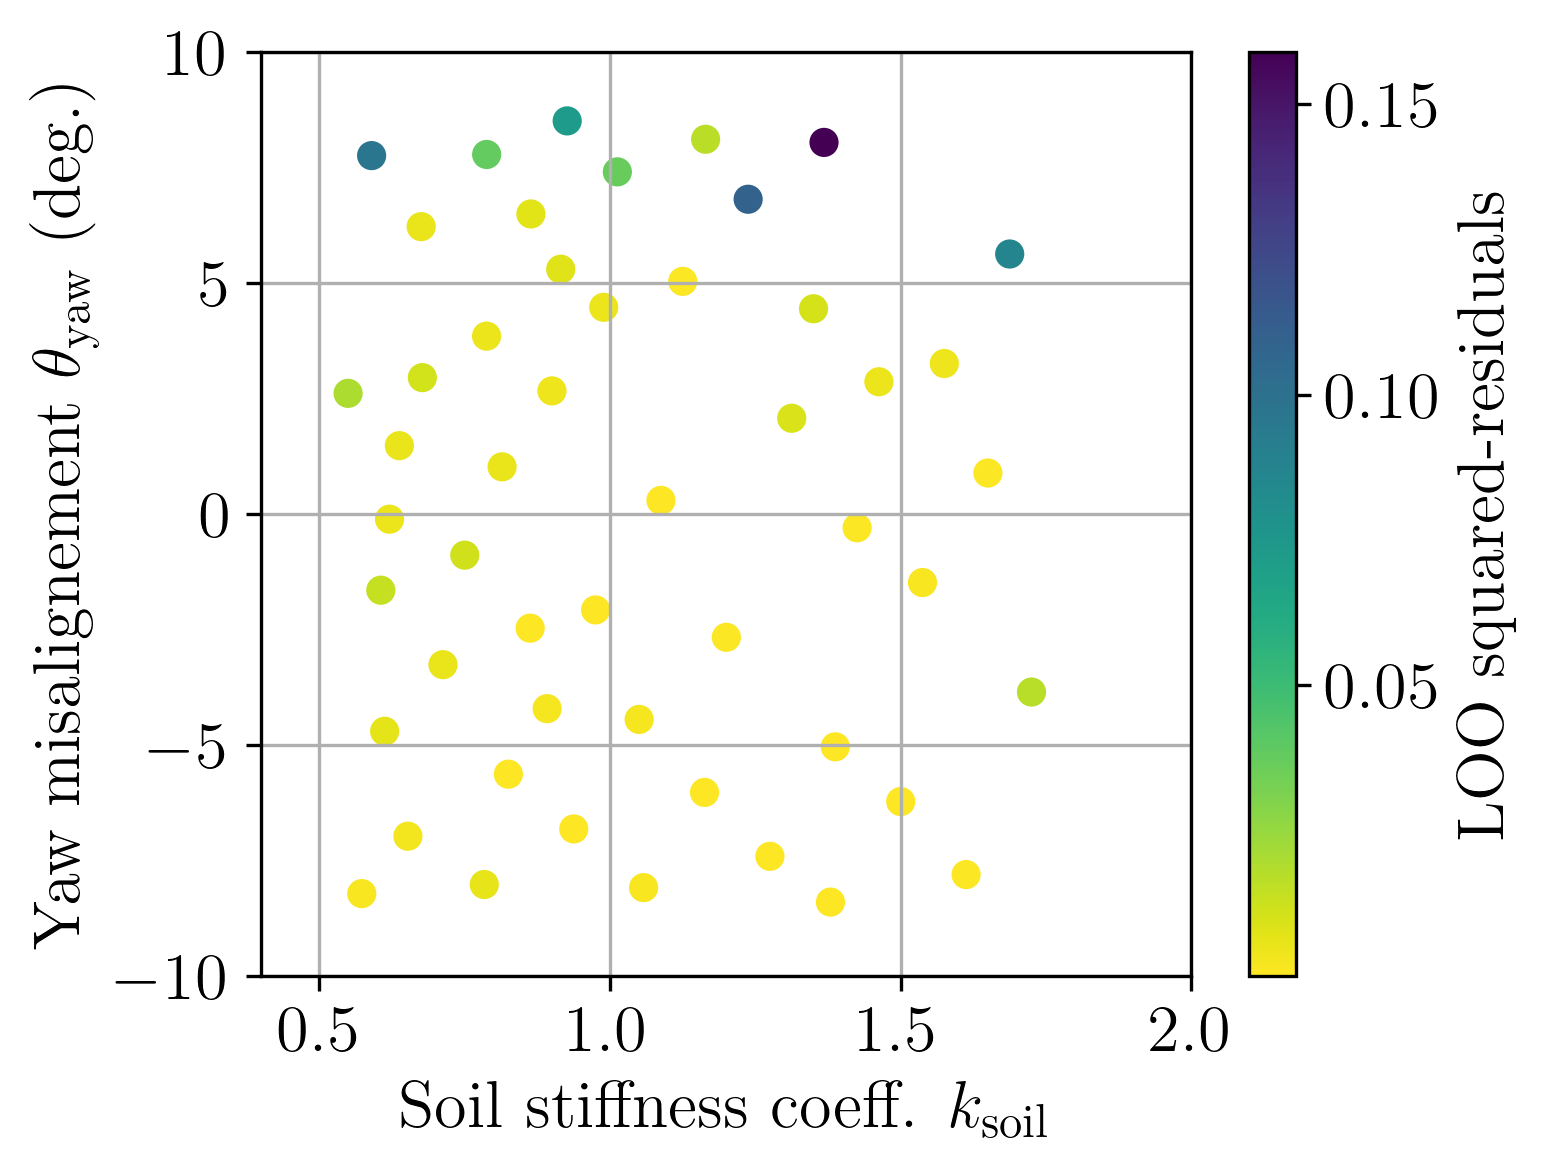
\includegraphics[width=\linewidth]{./part3/figures/OWT/loo_squared_res.png}
        \caption{LOO Squared-residuals.}
    \end{subfigure}
    \caption{Leave-one-out validation results of the surrogate model $\widetilde{D}$.}
    \label{fig:loo_validation}
\end{figure}

%============================================================%
%============================================================%
\section{Reliability and robustness analysis}
%============================================================%
%============================================================%
In the wind energy industry, acceptable risk levels for fatigue are defined by the standards. 
The target failure probability of the order of magnitude of $10^{-4}$ over the last year of exploitation is indicated by the \citet{iec_2019}. 
\citet{nielsen_2021_risk_levels} discussed the relevance of this risk level, defined from an economic point of view, and offered quantitative guidelines for lifetime extension. 
In this section, a probabilistic reliability analysis is conducted using the surrogate model of the lifetime cumulative damage. 
Afterwards, the robustness of this reliability analysis is studied by applying perturbations to the input distributions and computing the perturbed-law based sensitivity indices (PLI) initially proposed by \citet{lemaitre_2015_PLI}. 


%============================================================%
\subsection{Nominal reliability analysis}\label{sec:owt_ra}
%============================================================%

The surrogate model of the lifetime cumulative damage $\widetilde{D}$ is first modified to include the SN curve uncertainty $\varepsilon$, defined in Section~\ref{sec:probabilistic_sn}:
\begin{equation}
    \widetilde{D}'(\bz) = \widetilde{D}'(k_{\mathrm{soil}}, \theta_{\mathrm{yaw}}, \varepsilon) = \frac1\varepsilon \, \widetilde{D}(k_{\mathrm{soil}}, \theta_{\mathrm{yaw}}).
\end{equation} 
The probability introduced in \eq{eq:owt_pf} then becomes: 
\begin{equation}
    \pf = \int_{\iD_\bZ} \1_{\{\widetilde{D}'(\bz) \geq D_{\mathrm{cr}}\}} \, f_\bZ(\bz) \, \dd z \,,
    \label{eq:owt_pf_surrogate}
\end{equation}
Table~\ref{tab:pf_result_table} presents the estimates of this quantity by different methods (FORM, FORM-importance sampling and subset simulation, see Section~\ref{sec:reliability}) and for two hypotheses regarding the distribution of the resistance variable. 
$D_{\mathrm{cr}}$ either follows a lognormal distribution (which has a short left tail), or a normal distribution (with a heavier left tail). 
All the methods deliver similar values of $\pf$ even if subset simulation requires more time. 
The adequation of FORM with the simulation methods reveals that the limit-state function in this case is almost linear. 
Such a conclusion might differ depending on the OWT model studied (e.g., a floating model could present a different behavior). 
The probabilities are, as expected, much lower under the hypothesis of lognormal distribution for $D_{\mathrm{cr}}$ than for a normal distribution. 
However, this significant difference questions the robustness of this result to the probabilistic model of $D_{\mathrm{cr}}$ and $\bZ$.  

\begin{table*}[h]
    \centering
    \caption{Nominal reliability analysis (IS and SS size $N=5 \times 10^4$, SS $p_0=0.1$).}
    \begin{tabular}{r||c|c|c|c}
              &  \multicolumn{2}{c|}{$D_{\mathrm{cr}} \sim $ \bf Lognormal} & \multicolumn{2}{c}{$D_{\mathrm{cr}} \sim $ \bf Normal}\\
    \hline
    \bf Reliability method & $\widehat{\pf}$       & $\widehat{\mathrm{cov}}$    & $\widehat{\pf}$       & $\widehat{\mathrm{cov}}$ \\
    \hline\hline
    FORM      & $9.87 \times 10^{-13}$ & --                    & $3.35 \times 10^{-6}$ & --\\
    \hline
    FORM-IS   & $9.84 \times 10^{-13}$ & $1 \%$                & $3.36 \times 10^{-6}$ & $1 \%$\\
    \hline
    SS        & $9.46 \times 10^{-13}$ & $7 \%$               & $3.50 \times 10^{-6}$ & $4 \%$\\ 
    \end{tabular}
    \label{tab:pf_result_table}
\end{table*}


%============================================================%
\subsection{Robustness analysis using the perturbed-law sensitivity indices}\label{sec:owt_robustness}
%============================================================%
The method of \citet{lemaitre_2015_PLI}, later called \textit{perturbed-law based sensitivity indices} (PLI) by \citet{sueur_2017_PLI} relies on perturbating densities. 
The goal is to assess the robustness of a quantity of interest (a failure probability in our case) to these perturbations. 
An application of the PLI on a thermal-hydraulic numerical code from the nuclear industry was proposed in \citet{iooss_2022_pli}. 
\elias{Place the PLI in the robustness litterature?}

Assuming a random variable $Z_j \sim f_j \in \iD_{Z_j}$ with mean $\E[Z_j]=\mu$ and variance $\var(Z_j) = \sigma^2$, the strategy is to find the ``closest'' distribution $f_{j \delta}$ under the constraint of moment perturbation of magnitude $\delta$.  
The notion of proximity between distributions is quantified by \citet{lemaitre_2015_PLI} in terms of Kullback–Leibler divergence (KL). 
For example, a relative mean perturbation is defined as: 
\begin{eqnarray}
    f_{j \delta} = \argmin_{\substack{\pi\in \mathcal{P}, \\ \mathrm{s.t.}, \E_\pi[Z_j] = \E_{f_j}[Z_j](1 + \delta)}} \, \mathrm{KL}(\pi||f_j), \quad \delta \in \R. 
\end{eqnarray} 

Note that the perturbed distribution $f_{j \delta}$ might not belong to the parametric family of $f_j$. 
This is typically the case for bounded distributions, for example when perturbating the mean of a uniform distribution.  
To simplify the perturbation problem studied in \citet{lemaitre_2015_PLI, gauchy_2022_PLI}, the perturbations realized in the following will conserve the initial parametric family (which seems reasonable for distributions in the exponential family). 

The adapted expression of the PLI used hereafter \citep{gauchy_2022_PLI} reflects the relative impact of a pertubation on the quantity of interest: 
\begin{equation}
    \mathrm{PLI}(f_{j \delta}) = \frac{p_{\mathrm{f}, j \delta} - \pf }{\pf} \,,
\end{equation}
where $p_{\mathrm{f}, j \delta}$ is the probability obtained when injecting $f_{j \delta}$ in \eq{eq:owt_pf_surrogate}.

In our case, each variable in $\bZ$ is perturbed one by one in terms of relative standard deviation, such that $\sigma_{j \delta} = \sigma_j (1+\delta)$. 
The illustration of such perturbations is illustrated in \fig{fig:perturbations}, for distributions of $K_{\mathrm{soil}}$ on the left, and of $\Theta_{\mathrm{yaw}}$ on the right.
This strategy assumes that the analyst has enough information to determine the mean of the variables $Z_j$. 

The resulting PLI are presented in \fig{fig:pli_all} for relative perturbations of the standard deviations of $(K_{\mathrm{soil}}, \Theta_{\mathrm{yaw}}, \varepsilon)$. 
Each failure probability is independently estimated by FORM-IS. 
In the hypothesis of a normal $D_{\mathrm{cr}}$, the most important variable is $\Theta_{\mathrm{yaw}}$, while the fluctuations are quite stable in the hypothesis of a lognormal $D_{\mathrm{cr}}$. 

When perturbating the standard deviation of the resistance variable $D_{\mathrm{cr}}$, the same phenomenon is witnessed in \fig{fig:pli_resistance}. 
The perturbations have nearly no consequences, assuming that $D_{\mathrm{cr}}\sim \mathrm{LogNormal}$, but a lot of influence when $D_{\mathrm{cr}}\sim \mathrm{Normal}$.  
As a perspective, this study could be completed by a joint perturbation of both standard deviation and mean of the resistance variable.


\begin{figure}
    \centering
        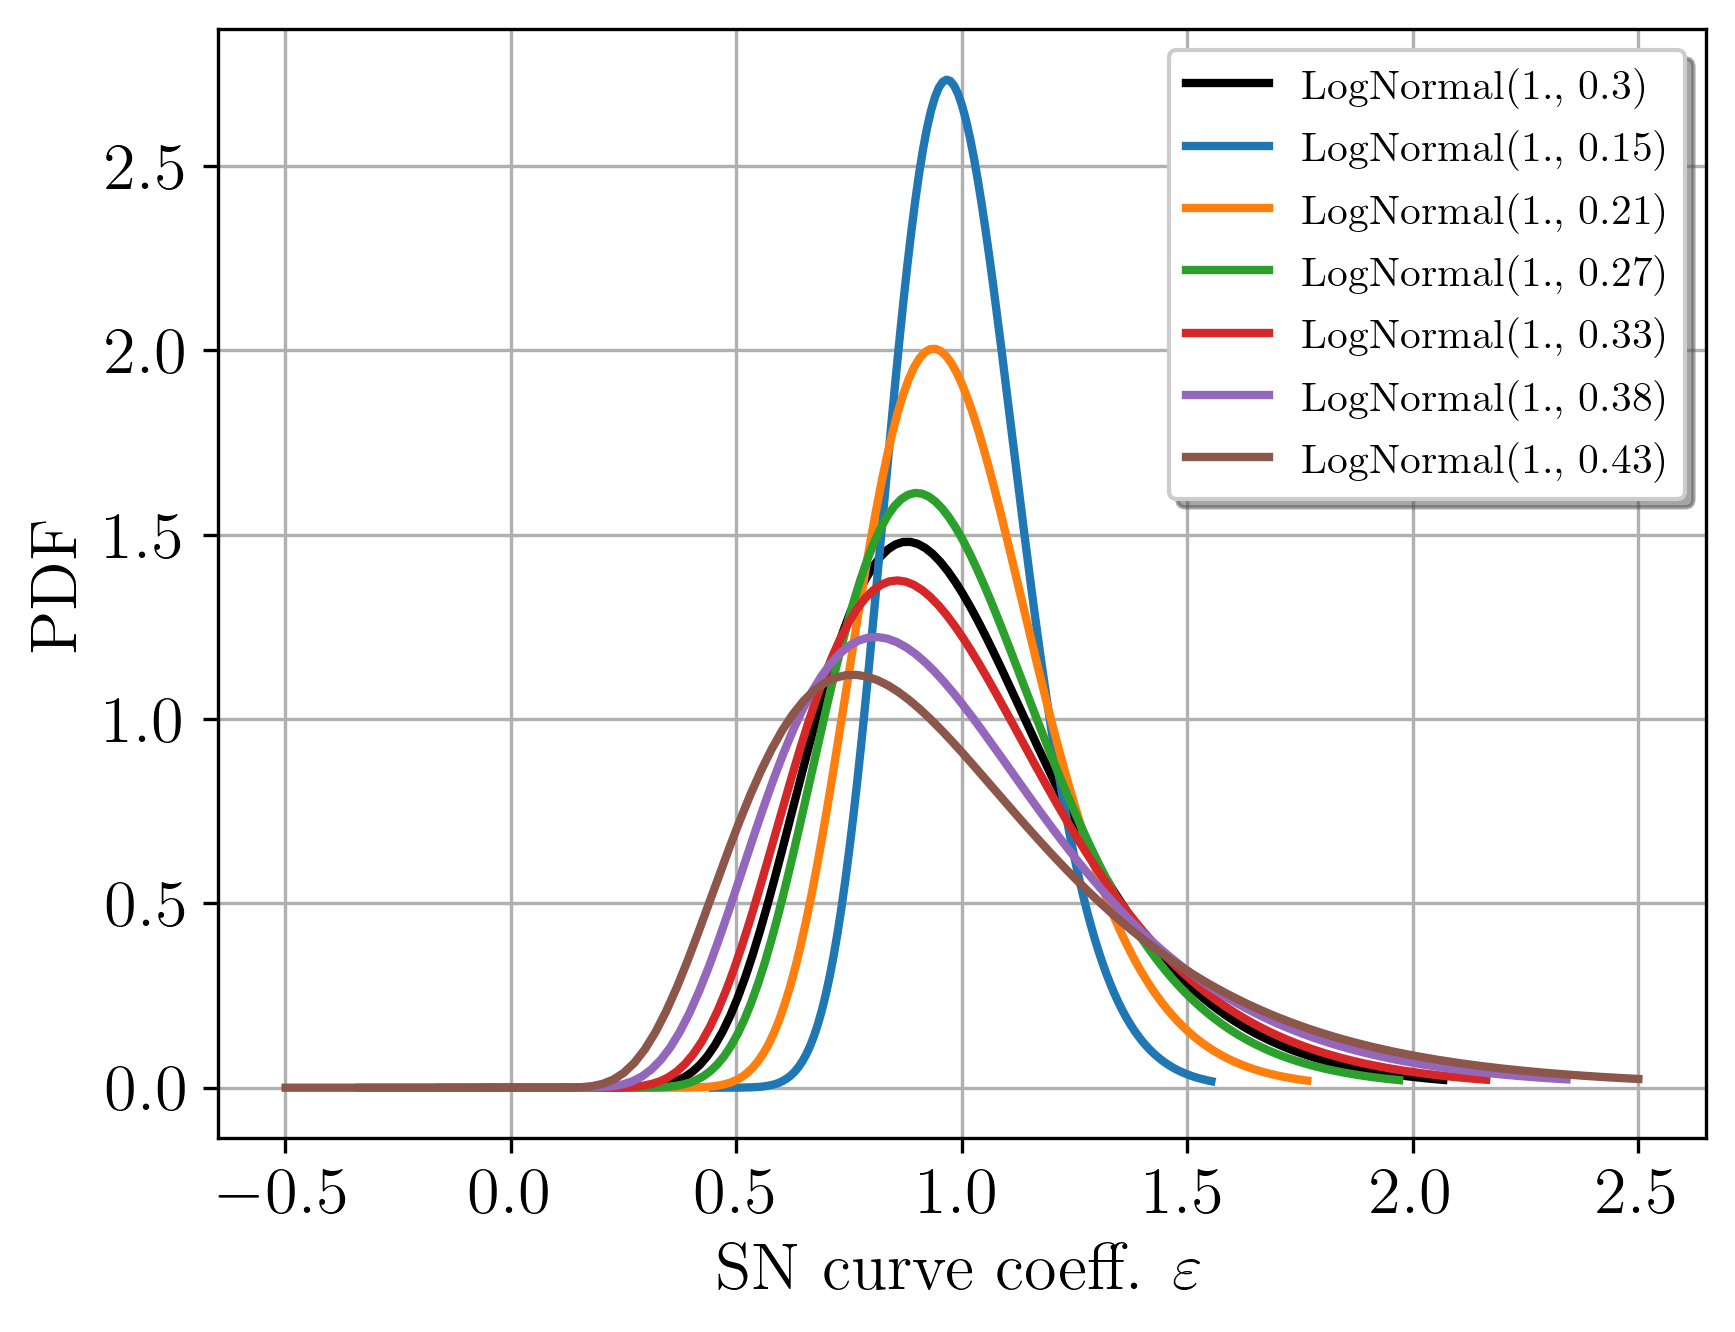
\includegraphics[width=0.43\linewidth]{./part3/figures/OWT/lognormal_pert.png}
        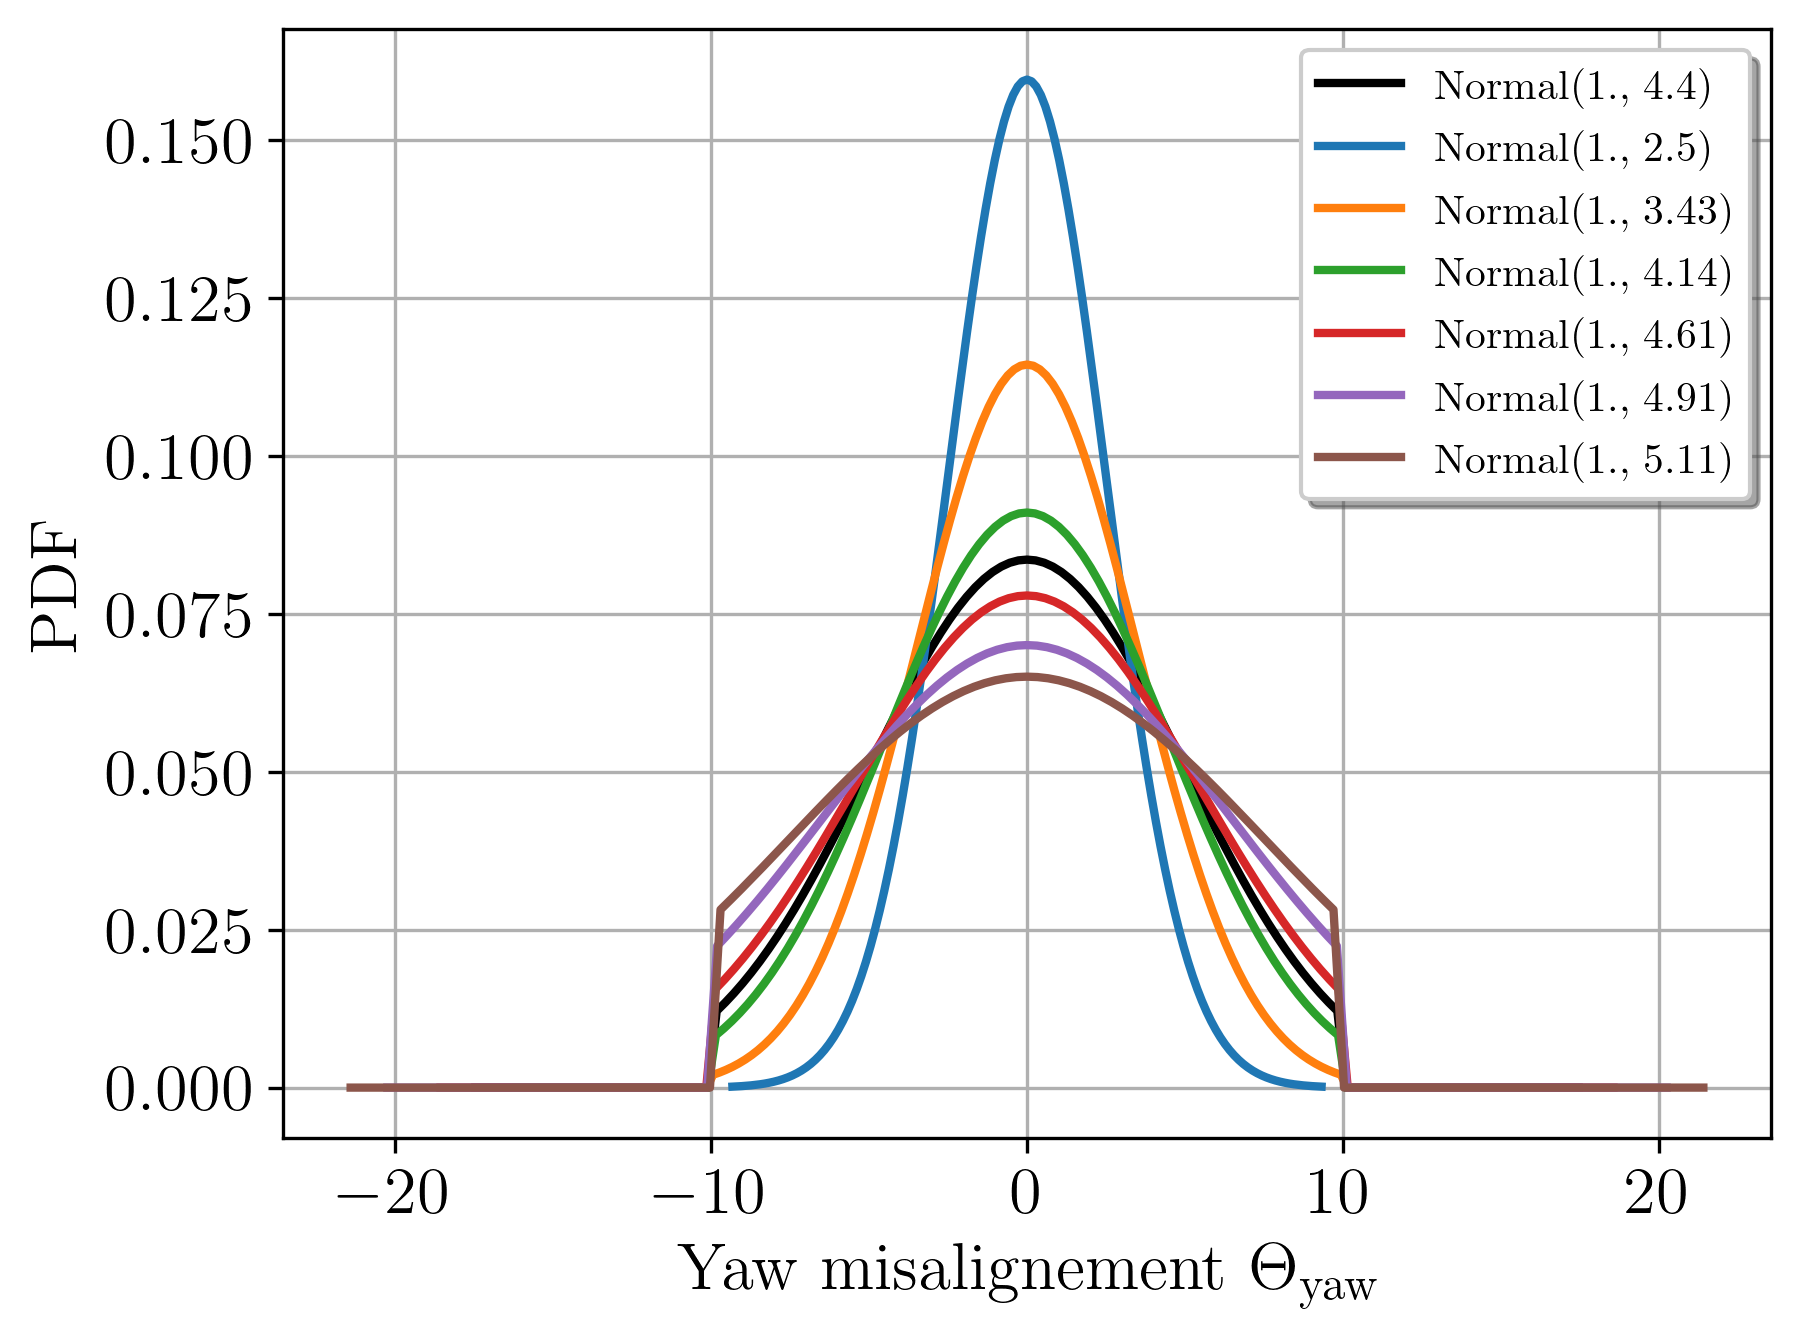
\includegraphics[width=0.44\linewidth]{./part3/figures/OWT/normal_pert.png}
    \caption{Perturbations in terms of standard deviation of a lognormal distribution (left) and a truncated normal distribution (right).}
    \label{fig:perturbations}
\end{figure}


\begin{figure}
    \centering
    \begin{subfigure}[t]{0.48\linewidth}
        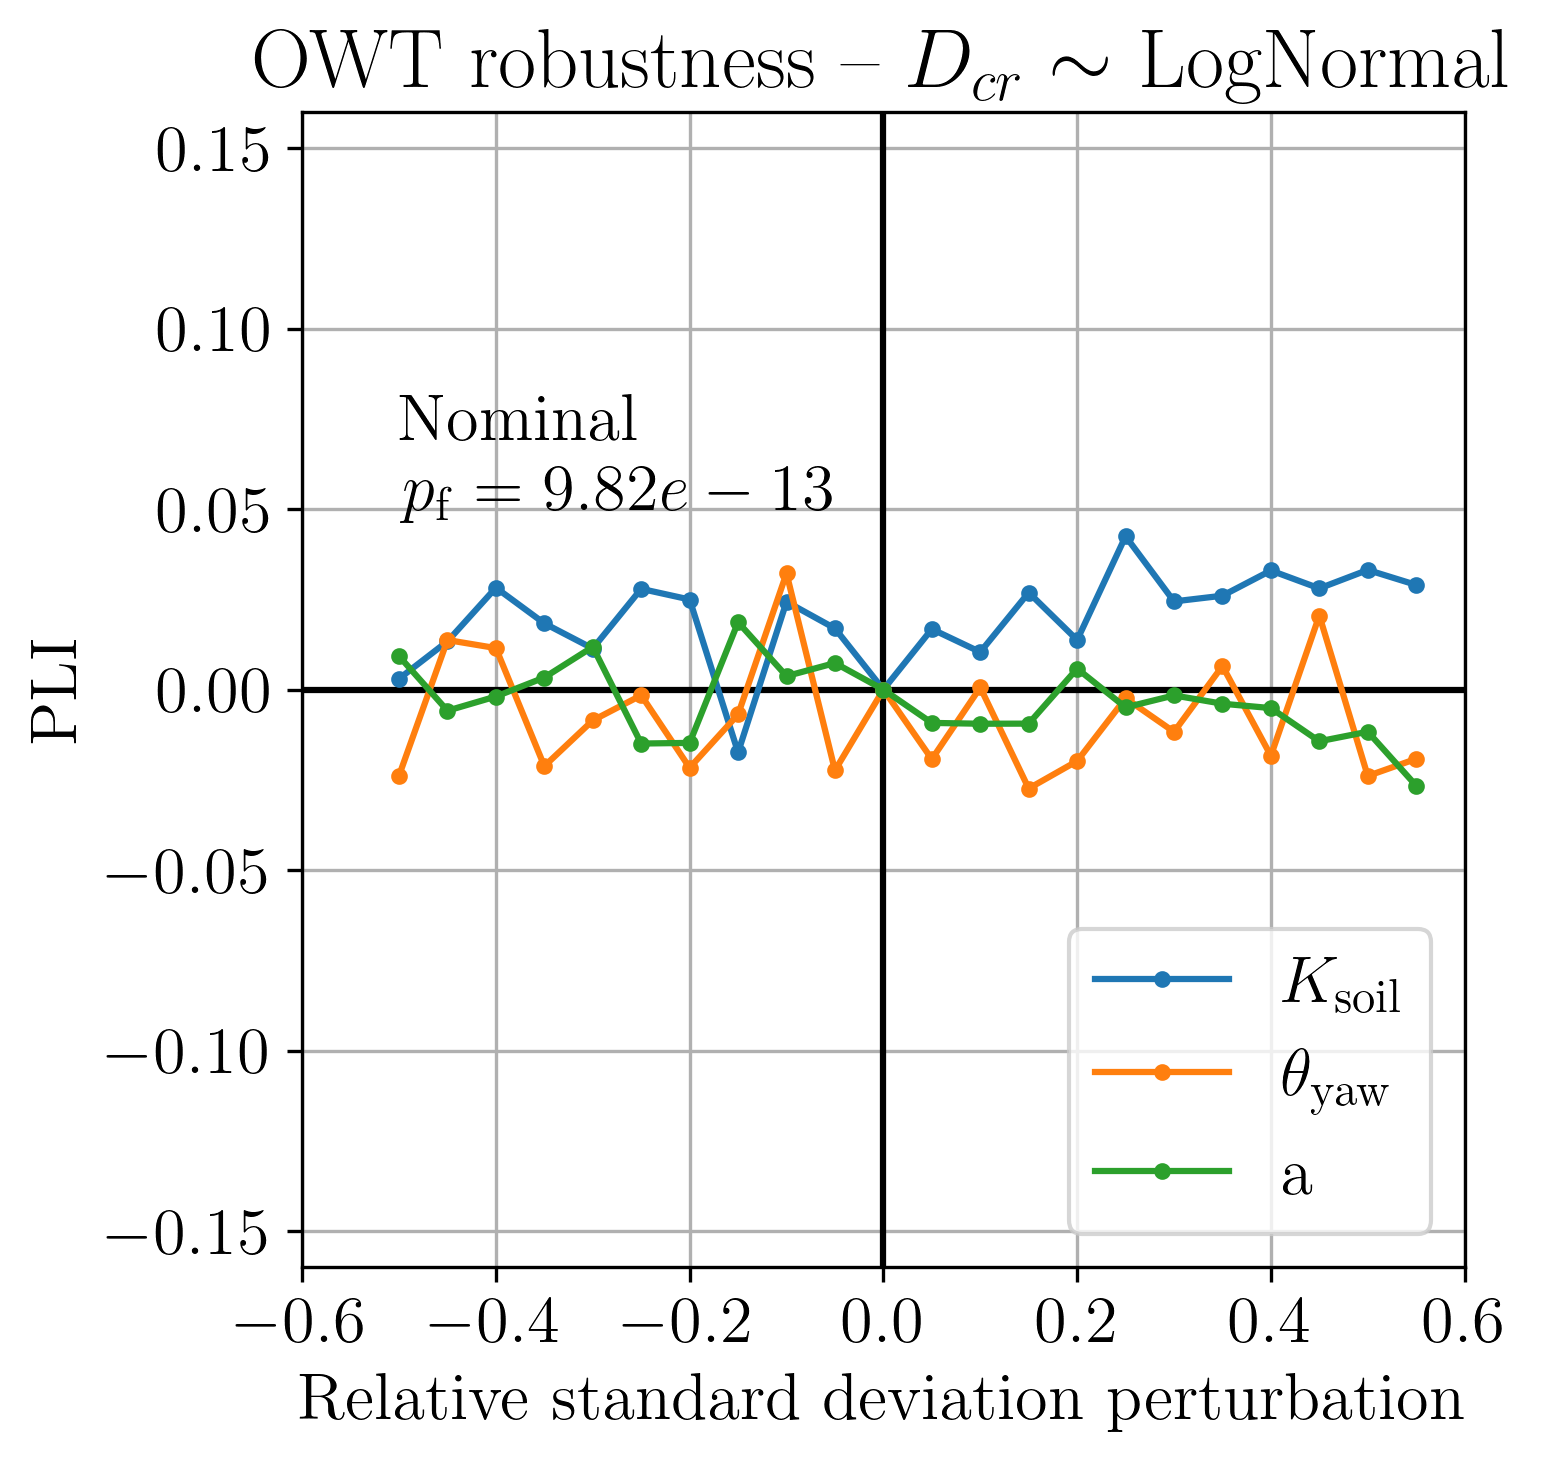
\includegraphics[width=\linewidth]{./part3/figures/OWT/PLI_ALL_Hyp_LogNormal.png}
        \caption{$D_{\mathrm{cr}} \sim $ Lognormal.}
    \end{subfigure}
    \begin{subfigure}[t]{0.48\linewidth}
        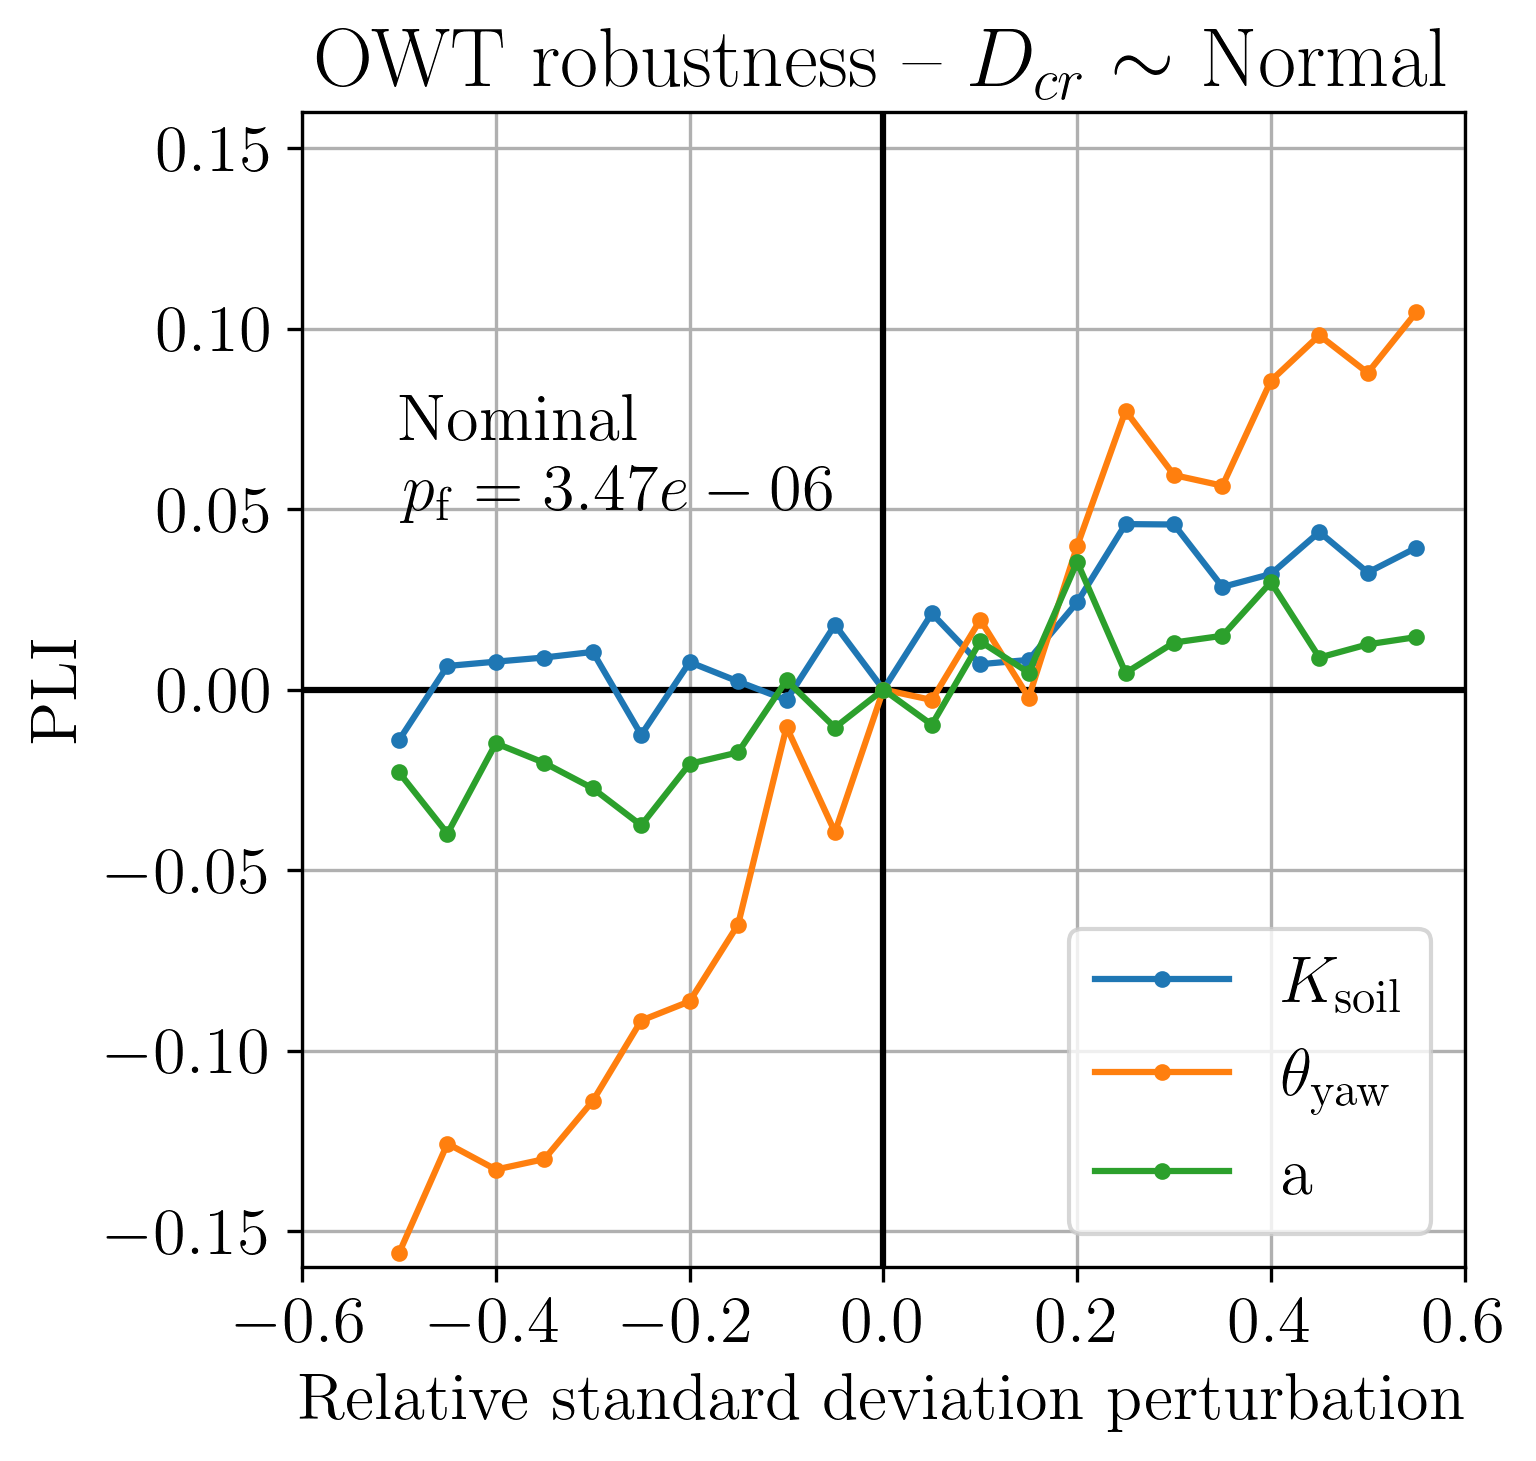
\includegraphics[width=\linewidth]{./part3/figures/OWT/PLI_ALL_Hyp_Normal.png}
        \caption{$D_{\mathrm{cr}} \sim $ Normal.}
    \end{subfigure}
    \caption{Perturbed-law based indices for relative perturbations of the standard deviations of $(K_{\mathrm{soil}}, \Theta_{\mathrm{yaw}}, \varepsilon)$. 
    The failure probabilities studied are each estimated by FORM-IS method with sample size $N=5 \times 10^4$.}
    \label{fig:pli_all}
\end{figure}


\begin{figure}
    \centering
    \begin{subfigure}[t]{0.48\linewidth}
        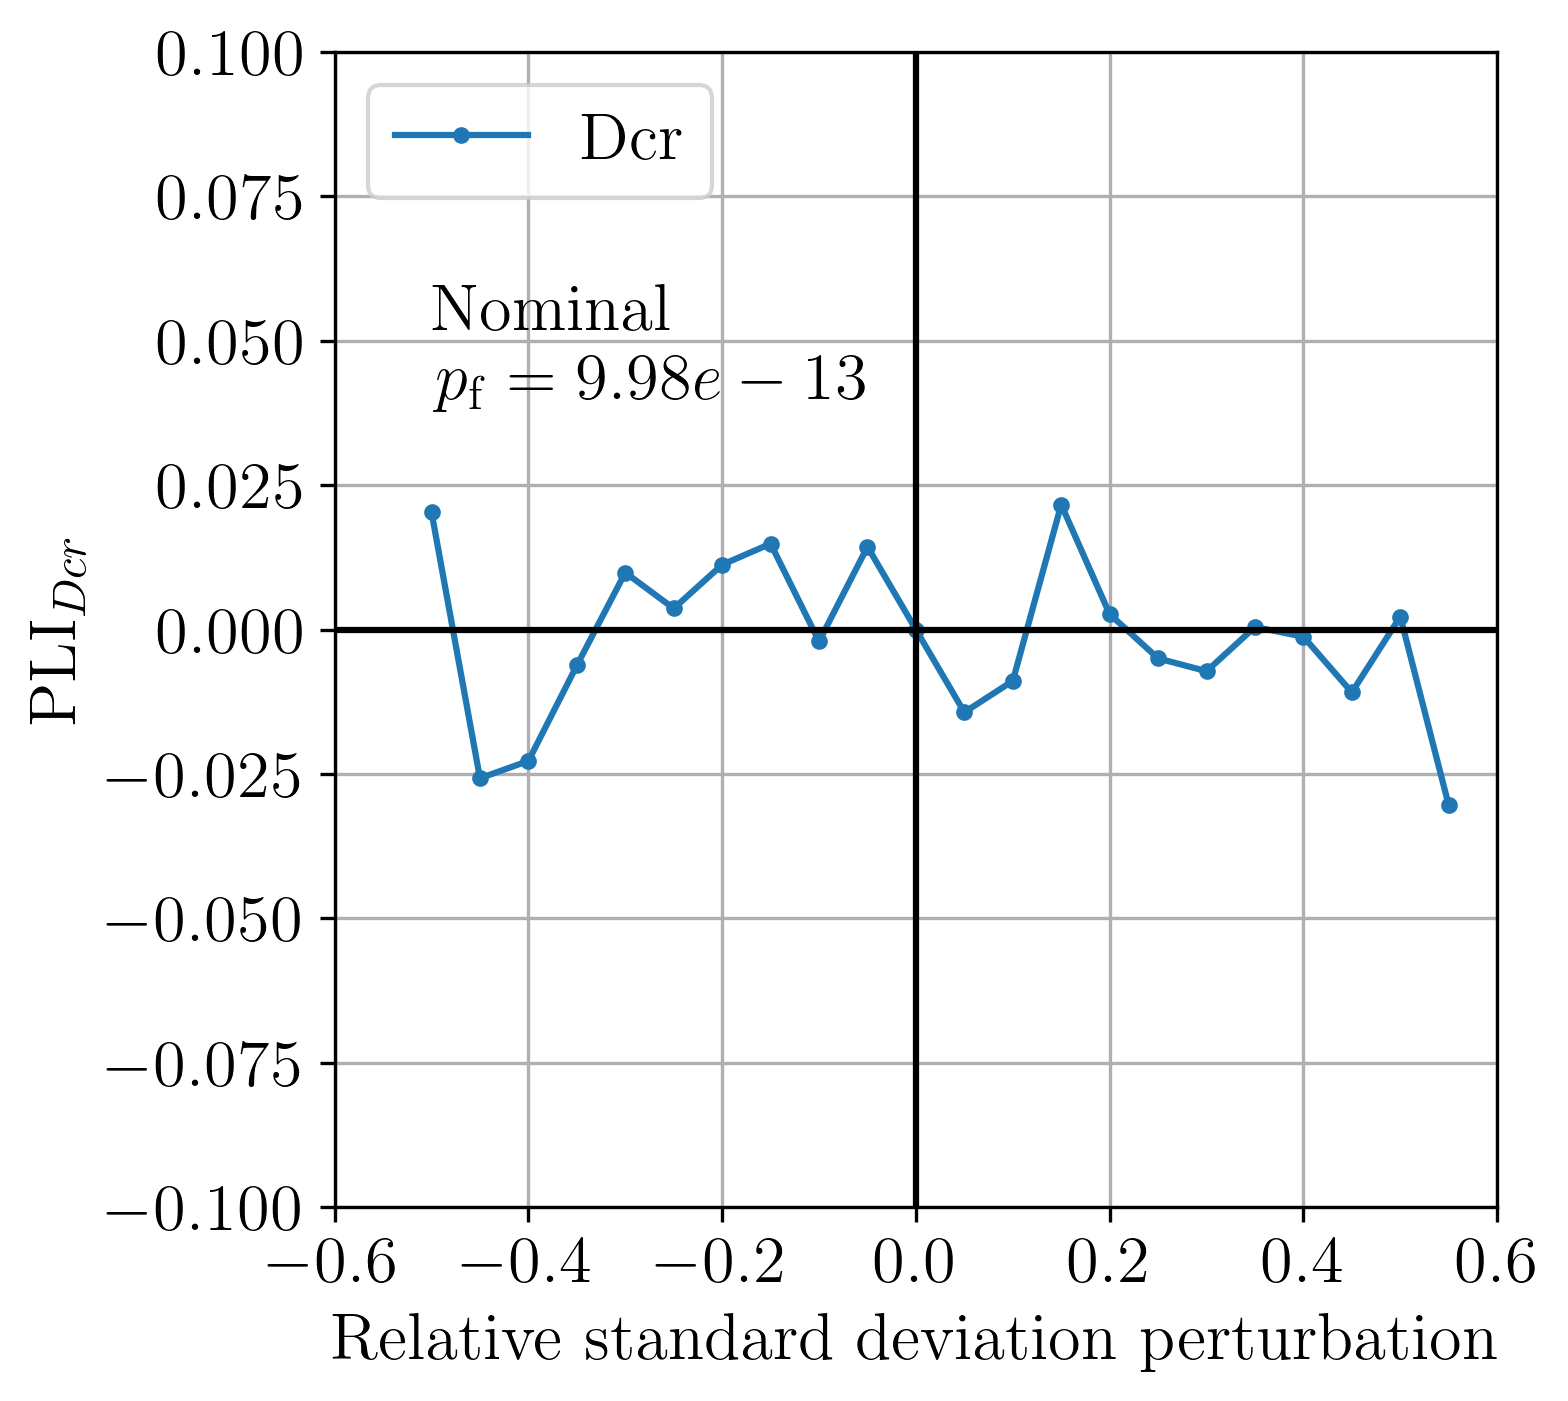
\includegraphics[width=\linewidth]{./part3/figures/OWT/PLI_Dcr_Hyp_LogNormal.png}
        \caption{$D_{\mathrm{cr}} \sim $ Lognormal.}
    \end{subfigure}
    \begin{subfigure}[t]{0.45\linewidth}
        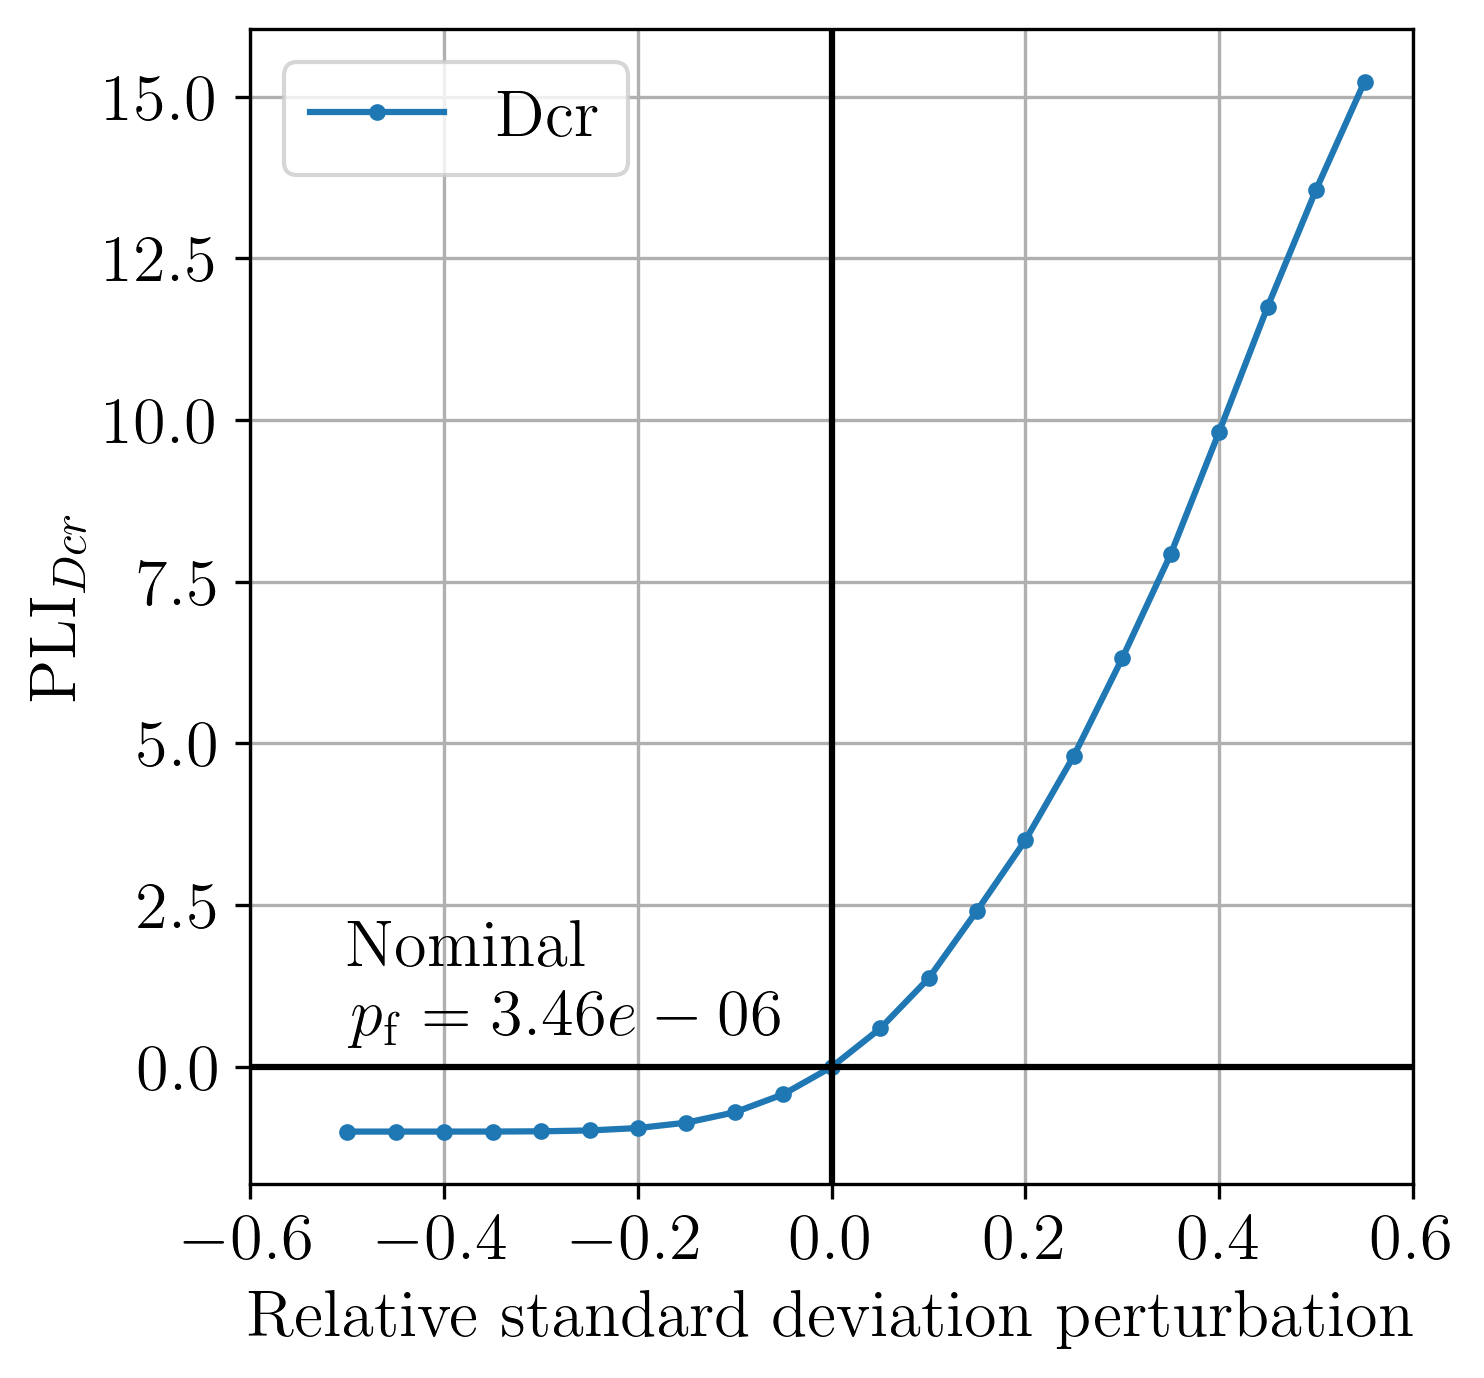
\includegraphics[width=\linewidth]{./part3/figures/OWT/PLI_Dcr_Hyp_Normal.png}
        \caption{$D_{\mathrm{cr}} \sim $ Normal.}
    \end{subfigure}
    \caption{Perturbed-law based indices for relative perturbations of the standard deviation of $D_{\mathrm{cr}}$. 
    The failure probabilities studied are each estimated by FORM-IS method with sample size $N=5 \times 10^4$.}
    \label{fig:pli_resistance}
\end{figure}

\newpage
%============================================================%
%============================================================%
\section{Conclusion}
%============================================================%
%============================================================%

In this chapter, a fully probabilistic reliability analysis was performed on the monopile foundation of an OWT located in Teesside, UK. 
Our demonstrative study first required an important computational effort (i.e., over $10^5$ Turbsim-DIEGO simulations), made possible with the development of a tailored wrapper deployed a high-performance facility. 
These simulations served the construction of a surrogate model emulating the lifetime damage function. 

The second phase of this chapter addressed the estimation of a failure probability using this surrogate. 
A general conclusion is that this probability is highly dependent of the probabilistic model describing the critical damage. 
To challenge the modeling hypothesis of the critical damage and the system variables, a robustness analysis was realized. 
It consists in studying the impact of perturbating the input distributions on an output quantity.   
The robustness of the failure probability was evaluated with the formalism of the perturbed-law based indices, introduced by \citet{lemaitre_2015_PLI}.
This additional study mostly confirmed the importance of the critical damage definition. 

From an industrial point of view, the failure probabilities obtained are much lower than, the risk levels targeted in the standards, which is in favor of lifetime extension. 
However, let us outline that this demonstrative results did not consider: 
\begin{itemize}
    \item The periods in parked position which could significantly increase the damage. 
    Different studies showed that the aerodynamic damping created by the rotation of the turbine reduces tower vibrations, and therefore fatigue \citep{liu_2017_damping};
    \item The rapid transition phases occasioned by emergency stopping;
    \item The early damage produced during the installation of the monopile foundations by hydraulic impact piling (i.e., hammering).  
    \item The stress-concentration resulting from soldering the structure;
\end{itemize} 
An interesting industrial perspective could be to reproduce a similar study on a floating OWT model and compare the conclusions.  

From a methodological aspect, a stochastic surrogate model could be built by considering all the damages before averaging them over the environmental repetitions. 
This framework would lead to the open question of reliability analysis on stochastic models \elias{add ref}. 
%\elias{http://www.tara.tcd.ie/bitstream/handle/2262/103570/submission_420.pdf?sequence=1}
%\elias{add the ref from T.Brown and other student from BIOOSS about quantiles and stochastic models}
